\documentclass{beamer}
\usepackage{cancel, algpseudocode, hyperref, tikz, venndiagram, centernot}

\title{CS 70 Discussion 2B}
\date{September 13, 2024}

\begin{document}

\frame{\titlepage}

\begin{frame}
    \frametitle{Graphs}
    Graph definitions (some requirements are specific to this class):
    \begin{itemize}
        \item {\bf Vertices/Nodes} (typically denoted as circles/squares)
        \item {\bf Edges} (either {\bf directed} or {\bf undirected}, and are denoted as lines between two nodes)
        \item Maximum of one edge between each pair of nodes (max one in each direction for directed graph)
        \item No edge from a node back to itself ({\bf self-loop})
    \end{itemize}
    Examples of valid graphs:\\
    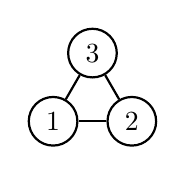
\begin{tikzpicture}[-,auto,node distance=3cm,thick,main node/.style={circle,draw},scale=0.5]
        \node [circle, draw] (1) at (0,0) {1};
        \node [circle, draw] (2) at (2,0) {2};
        \node [circle, draw] (3) at (1, 1.732) {3};
        \path[every node]
        (1) edge node [right, above] {} (2)
        (2) edge node [below] {} (3)
        (3) edge node [left, above] {} (1);
    \end{tikzpicture}
    \hspace{5pt}
    \begin{tikzpicture}[->,auto,node distance=3cm,thick,main node/.style={circle,draw},scale=0.5]
    
        \node[main node] (4) {1};
        \node[main node, yshift=-45pt] (2) [above right of=1] {2};
        \node[main node, yshift=45pt] (3) [below right of=1] {3};
        \node[main node, xshift=40pt] (4) [right of=1] {4};
        
        \path[draw] (1) edge (2);
        \path[draw] (2) edge [bend left=15] (4);
        \path[draw] (4) edge [bend left=15] (2);
        \path[draw] (1) edge (3);
        \path[draw] (3) edge (4);

    \end{tikzpicture}\\
    Examples of invalid graphs:\\
    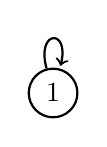
\begin{tikzpicture}[-,auto,node distance=3cm,thick,main node/.style={circle,draw},scale=0.5]
        \node[main node] (1) {1};
        \path[draw, loop above]
        (1) edge (1);
    \end{tikzpicture}
    \hspace{5pt}
    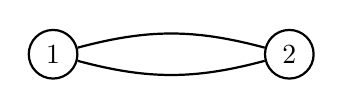
\begin{tikzpicture}[-,auto,node distance=3cm,thick,main node/.style={circle,draw},scale=0.5]
        \node[main node] (1) {1};
        \node[main node] (2) [right of=1] {2};
        \path[draw] (1) edge [bend left=15] (2);
        \path[draw] (2) edge [bend left=15] (1);
    \end{tikzpicture}
    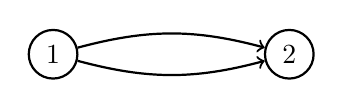
\begin{tikzpicture}[->,auto,node distance=3cm,thick,main node/.style={circle,draw},scale=0.5]
        \node[main node] (1) {1};
        \node[main node] (2) [right of=1] {2};
        \path[draw] (1) edge [bend left=15] (2);
        \path[draw] (1) edge [bend right=15] (2);
    \end{tikzpicture}
\end{frame}

\begin{frame}
    \frametitle{Graphs (Cont.)}
    {\bf Degree}: Number of edges connected to a particular vertex
    \begin{itemize}
        \item {\bf Handshake Lemma}: $\sum_{v\in V}\text{deg}(v)=2|E|$ ($E$ is the set of all edges in the graph, $V$ is the set of all vertices in the graph, and $\deg$ is a function that gives us the degree of a specific vertex)
        \item Directed graphs: {\bf in-degree} (number of edges going into a vertex) and {\bf out-degree} (number of edges going out of a vertex)
    \end{itemize}
    Types of graph traversals:
    \begin{itemize}
        \item {\bf Walk}: Start at some node and move between nodes using edges
        \item {\bf Path}: Same as a walk, but cannot revisit edges or vertices
        \item {\bf Tour}: Same as a walk, but starts and ends at the same vertex
        \item{\bf Cycle}: Same as a tour, but cannot revisit edges or vertices (except for the starting/ending vertex)
    \end{itemize}
\end{frame}

\begin{frame}
    \frametitle{Graphs (Cont.)}
    {\bf Connected Component}: A set of vertices in a graph where every vertex in the set can visit any other vertex in the set through some path (ex: the connected components of the below graph are $\{1,2,3\}$ and $\{4,5\}$)\\
    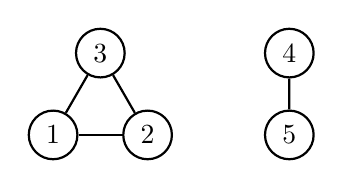
\begin{tikzpicture}[-,auto,node distance=3cm,thick,main node/.style={circle,draw},scale=0.6]
        \node [circle, draw] (1) at (0,0) {1};
        \node [circle, draw] (2) at (2,0) {2};
        \node [circle, draw] (3) at (1, 1.732) {3};
        \node [circle, draw] (4) at (5,1.732) {4};
        \node [circle, draw] (5) at (5,0) {5};
        \path[every node]
        (1) edge node [right, above] {} (2)
        (2) edge node [below] {} (3)
        (3) edge node [left, above] {} (1)
        (4) edge node [below] {} (5);
    \end{tikzpicture}
\end{frame}

\begin{frame}
    \frametitle{Eulerian Tour/Walks}
    \begin{enumerate}[-]
        \item {\bf Eulerian Tour}: A tour that visits every edge in the graph exactly once
        \item {\bf Eulerian Walk}: A walk that visits every edge in the graph exactly once
        \item {\bf Condition 1}: An Eulerian tour exists iff all degrees in the graph are even:
        \begin{enumerate}[-]
            \item An Eulerian tour can be started from any vertex!
            \item There is an algorithm that can find an Eulerian tour in a graph quickly (if it exists)
        \end{enumerate}
        \item {\bf Condition 2}: An Eulerian walk exists iff all degrees in the graph are even except for exactly $2$ odd-degree vertices:
        \begin{enumerate}[-]
            \item The Eulerian walk must start at one of the odd-degree vertices
            \item There is an algorithm that can find an Eulerian walk in a graph quickly (if it exists)
        \end{enumerate}
    \end{enumerate}
\end{frame}

\begin{frame}
    \frametitle{Trees}
    There are three {\it equivalent} definitions for a tree:
    \begin{itemize}
        \item A connected graph with no cycles
        \item A connected graph with $n-1$ edges ($n$ is number of vertices)
        \item A connected graph where removing any edge splits graph into multiple connected components
    \end{itemize}
    Ex:\\
    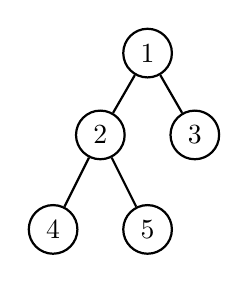
\begin{tikzpicture}[-,auto,node distance=3cm,thick,main node/.style={circle,draw},scale=0.6]
        \node [circle, draw] (2) at (0,2) {2};
        \node [circle, draw] (3) at (2,2) {3};
        \node [circle, draw] (1) at (1,3.732) {1};
        \node [circle, draw] (4) at (-1,0) {4};
        \node [circle, draw] (5) at (1,0) {5};
        \path [draw] (1) edge (2);
        \path [draw] (1) edge (3);
        \path [draw] (2) edge (4);
        \path [draw] (2) edge (5);
    \end{tikzpicture}
\end{frame}

\begin{frame}
    \frametitle{Graph Coloring}
    {\bf Vertex Coloring Problem}: Color all vertices of a graph using $k$ colors such that no adjacent vertices have the same color. Ex:\\
    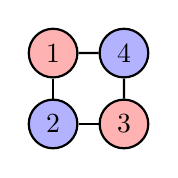
\begin{tikzpicture}[-,auto,node distance=3cm,thick,main node/.style={circle,draw},scale=0.6]
        \node [circle, draw, fill=red!30] (1) at (0,1.5) {1};
        \node [circle, draw, fill=blue!30] (2) at (0,0) {2};
        \node [circle, draw, fill=red!30] (3) at (1.5,0) {3};
        \node [circle, draw, fill=blue!30] (4) at (1.5,1.5) {4};
        \path [draw] (1) edge (2);
        \path [draw] (2) edge (3);
        \path [draw] (3) edge (4);
        \path [draw] (4) edge (1);
    \end{tikzpicture}\\
    {\bf Edge Coloring Problem}: Color all edges of a graph using $k$ colors such that no adjacent edges have the same color. Ex:\\
    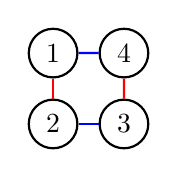
\begin{tikzpicture}[-,auto,node distance=3cm,thick,main node/.style={circle,draw},scale=0.6]
        \node [circle, draw] (1) at (0,1.5) {1};
        \node [circle, draw] (2) at (0,0) {2};
        \node [circle, draw] (3) at (1.5,0) {3};
        \node [circle, draw] (4) at (1.5,1.5) {4};
        \path [draw=red] (1) edge (2);
        \path [draw=blue] (2) edge (3);
        \path [draw=red] (3) edge (4);
        \path [draw=blue] (4) edge (1);
    \end{tikzpicture}
\end{frame}

\end{document}